\documentclass[11pt, a4paper, leqno]{article}
\usepackage{a4wide}
\usepackage[T1]{fontenc}
\usepackage[utf8]{inputenc}
\usepackage{float, afterpage, rotating, graphicx}
\usepackage{epstopdf}
\usepackage{longtable, booktabs, tabularx}
\usepackage{fancyvrb, moreverb, relsize}
\usepackage{eurosym, calc}
% \usepackage{chngcntr}
\usepackage{amsmath, amssymb, amsfonts, amsthm, bm}
\usepackage{caption}
\usepackage{mdwlist}
\usepackage{xfrac}
\usepackage{setspace}
\usepackage[dvipsnames]{xcolor}
\usepackage{subcaption}
\usepackage{minibox}
%\usepackage{natbib}
%\usepackage{bookmark}
%\usepackage{natbib}
%\usepackage{biblatex}
% \usepackage{pdf14} % Enable for Manuscriptcentral -- can't handle pdf 1.5
% \usepackage{endfloat} % Enable to move tables / figures to the end. Useful for some
% submissions.

\usepackage[
    natbib=true,
    bibencoding=inputenc,
    bibstyle=authoryear-ibid,
    citestyle=authoryear-comp,
    maxcitenames=3,
    maxbibnames=10,
    useprefix=false,
    sortcites=true,
    backend=biber
]{biblatex}
\AtBeginDocument{\toggletrue{blx@useprefix}}
\AtBeginBibliography{\togglefalse{blx@useprefix}}
\setlength{\bibitemsep}{1.5ex}
\addbibresource{../../paper/refs.bib}

\usepackage[unicode=true]{hyperref}
\hypersetup{
    colorlinks=true,
    linkcolor=black,
    anchorcolor=black,
    citecolor=NavyBlue,
    filecolor=black,
    menucolor=black,
    runcolor=black,
    urlcolor=NavyBlue
}
% \usepackage[
%     authordate,autocite=inline,backend=biber,sorting=nyt,natbib=true]{biblatex}
\widowpenalty=10000
\clubpenalty=10000

\setlength{\parskip}{1ex}
\setlength{\parindent}{0ex}
\setstretch{1.5}



% \usepackage[unicode=true]{hyperref}
% \hypersetup{
%     colorlinks=true,
%     linkcolor=black,
%     anchorcolor=black,
%     citecolor=NavyBlue,
%     filecolor=black,
%     menucolor=black,
%     runcolor=black,
%     urlcolor=NavyBlue
% }


% \widowpenalty=10000
% \clubpenalty=10000

% \setlength{\parskip}{1ex}
% \setlength{\parindent}{0ex}
% \setstretch{1.5}


\begin{document}

\title{Elevating Trust by increasing Instruction hours-German G8 Reform \thanks{Adrija Roy, University of Bonn. Email: \href{mailto:s6adroyy@uni-bonn.de}{\nolinkurl{s6adroyy [at] uni-bonn [dot] de}}.}}

\author{Adrija Roy}

\date{
    %{\bf Preliminary -- please do not quote}
    %\\[1ex]
    \today
}

\maketitle

\begin{abstract}
    For this project I examine the the effect of a major German high school implemented 
    between 2001 and 2008 in most of the federal States on student's trust attitude. The 
    reform reduced the secondory education by one year from 9 to 8 which lead to the increase
    in the weekly instruction hours. Since the policy G8 reform was implemented in diffrent 
    time over the period of 7 years I use difference in difference approach with time as 
    year of high school entry and State as fixed effects. I get a significant reult on 
    students' trust attitude. I also tried to look into some of the potential mechanisms 
    in line with other existing literatures.  
    
\end{abstract}

\clearpage


\section{Introduction\label{sec:introduction}}
A growing body of emperical literature has emphasized trust plays important role 
in economic development and direct efect on total factor productivity.\autocite{knack1997does}.
At the individual level, there is evidence linking trust and subjective well-being.\citep{helliwell2010trust}. 
Education plays a crucial role in shaping children's trust behavior in a positive way,\citep{glaeser2007does}.  
Raising instruction time in high school is often considered with having several positive effects for students'
outcomes,  especially regarding improvements in cognitive skills and performance.\citep{huebener2017increased}  
and eventually making schooling more efficient.  Even though many countries are attracted by the idea of 
reaping the benefits of increased instruction time in school \citep{oecd2016},outcomes other than student performance 
might be affected as well.\citep{dahmann2014impact,dahmann2018cross}.\par
Here aim is to analyse whether higher instruction hours affected students' self rated trust, 
measured as trust in people and strangers.The remainder of the paper is structured as follows. 
In Section\ref{sec:literature} provides some literatures overview on different outcomes affected 
by schooling and also review existing literature on the German G8-reform whereas 
Section\ref{sec:reform} briefly summarizes the main characteristics and features of the 
very reform. Afterwards, Section\ref{sec:data} introduces the data set used and
Section\ref{sec:strategy} gives reasoning on empirical strategy and lastly a short description 
of the results\ref{sec:results} and\ref{sec:conclusion}. Below the appendix section shows the graph for 
the treatement status with recpect to the variables used and the tables described in the paper. 

\section{Related literature\label{sec:literature}}
On the determinants of trust,\citep{alesina2002trusts}argue that individual experiences like 
traumatic events or (historically rooted) discrimination as well as one's community environment are 
among the strongest factors reducing trust.Accordingly \citep{glaeser1999social}find less trustworthy
behavior between people from different races or nationalities what has also been shown by 
\citep{Borgonovi2012} in a cross-European country comparison. \citep{dohmen2008representative} 
using 2003 and 2005 waves of the SOEPdata set, that female people, elderly as well as tall ones 
are usually associated with exhibiting more trust. On the other hand, trust seems to be strongly 
connected to personality traits as shown by \citep{dohmen2008representative} and 
\citep{becker2012relationship}. The former authors examine the effect of psychological traits as 
measured by the ``Big Five''concept and argue that more conscientious or more neurotic people 
trust less whereas individuals who are more agreeable or more open to experiences tend to trust more.
\par Moreover, there exists some evidence that schooling might affect social preferences 
including trust as well as altruism and reciprocity. Focusing on the effect of schooling on an 
individual's trust formation, current literature usually indicates that schooling and education 
in general have a positive impact on individual trust attitudes (see for example\citep{oreopoulos2011priceless}).

\section{The G8 reform\label{sec:reform}}
The G8 reform analyzed in this study affects only one of these tracks, the academic high school (\textit{Gymnasium}), 
which constitutes the high-ability school track that upon competition leads to the Abitur, the university entrance 
qualification that is required for admission to the university. Typically, academic high school lasted nine years, 
implying a total of thirteen years of schooling. Between 2001 and 2008, 13 out of 16 German federal states reduced 
the length of academic track schooling from nine to eight years reducing overall schooling from 13 to 12 years.
most of the additional workload usually being concentrated between grades seven to nine thus students are especially 
exposed to a higher workload between ages 13 and 16 (see for example \citep{dahmann2014impact, dahmann2018cross}).


\section{Data\label{sec:data}}
Analysis is based on a sample of same-aged students taken from the German Socio-Economic Panel (SOEP) study, a 
representative household panel survey.\footnote{Use data from the SOEP, data for years 1984-2020, version 37,
SOEP, 2021.}Adolescents, who respond to the SOEP youth questionnaire in the year they turn seventeen, answer survey 
questions relating to trust preferences in every wave starting in 2006. Hence, restricted to the data from 2006 through 2018, 
\footnote{Exclude data of recent immigrants and refugee samples.Also exclude data from 2019 and 2020 since some 
states swished back to the G9 scheme} and select all adolescents who were attending academic high school (\textit{Gymnasium}) 
at the time of the survey or had earned a high school diploma.\par To identify whether a student is subject to higher school intensity, 
used the information on the federal state of residence and the year of high-school entry. In case information on the latter is not provided, 
the year of high-school entry is imputed from the date of birth. Exclude students from Rhineland-Palatine where the reform has not been implemented 
state-wide, and students from Hesse who entered academic high school in 2004 and 2005 when schools operated under both schemes (G8 and G9). Individuals who
repeated one or more grades is also excluded to avoid noise from different levels of schooling experienced.\par \textbf{Trust.} Standard trust 
questions were included using three statements about whether “people can be generally trusted,” whether “nowadays one can’t rely on anyone,” 
and whether “if dealing with strangers, it is better to be careful before trusting them.” Answers were given on a seven-point Likert scale ranging 
from “agree completely” to “totally disagree.” collapsed multiple measures of trust into one index and standardized it so that, by construction, trust 
has a mean zero and a standard deviation of one.  

\section{Empirical strategy\label{sec:strategy}}

In order to estimate a causal effect of schooling intensity on trust, we exploit the aforementioned G8 reform, in particular,  we exploit the fact that 
the reform was implemented at different points in time across federal states. We apply a difference-in-differences strategy of the following form   
\begin{equation}
   y_{ist}= \gamma_{s} + \tau_{t} + \alpha G8_{st} + \beta X_{ist} +  \epsilon_{ist}
   \label{eqn:main_eqn}
\end{equation}
where $y_{ist}$ is the degree of trust at age 17 of student $i$ living in state $s$ who has entered high school at time $t$. $G8_{st}$ is a binary variable 
that identifies whether the student was affected by the G8 reform. Control group are students who entered academic high school before the reform yeras and graduate 
after nine years of high school, i.e., facing a lower schooling intensity. In contrast, our treatment group comprises students who entered academic high school 
after the reform and graduate after only eight years of academic high school, i.e., facing a higher schooling intensity. $\alpha$ is the coefficient of core interest 
and provides the reform's effect on student's trust. $\gamma_{s}$ is a set of state fixed effects that captures general differences between states, like time constant 
differences in state's education systems. A set of time fixed effects ($\tau_{t}$) capture general differences between cohorts over time as well as student trust shocks 
common to all federal states, e.g.resulting from policy changes applying to all federal states.\par The set of individual control variables $X_{ist}$ contains gender, 
childhood environment, previous educational performance, parental education dummy (at least one parent has an academic high school degree or higher), father's occupational status 
dummy (blue-collar occupation), the employment status of the mother and a dummy for being raised by a single parent, religion dummy.  Finally $\epsilon_{ist}$ is the error term. 
As the error term is likely to be correlated within states, following the recommendation of \citep{bertrand2004much} and cluster the standard errors at the level 
of the policy change.

\section{Results\label{sec:results}}
\subsection{Graphical evidence}
Figure\ref{fig:event_study} in the appendix depicts a graphical illustration of the reform's effect on trust. As the reform was implemented at different points of time, 
the estimated event study-style specifications with saturated leads and lags. I have used four lags periods and seven leads. Although the graph doesnot totally provide 
the validity of event study, I sticked to this for the purpose of theis project. What can be noticed is the positive effct of trust post reform which also matches the 
result of main regression table. 

\begin{figure}[H]
    \centering
    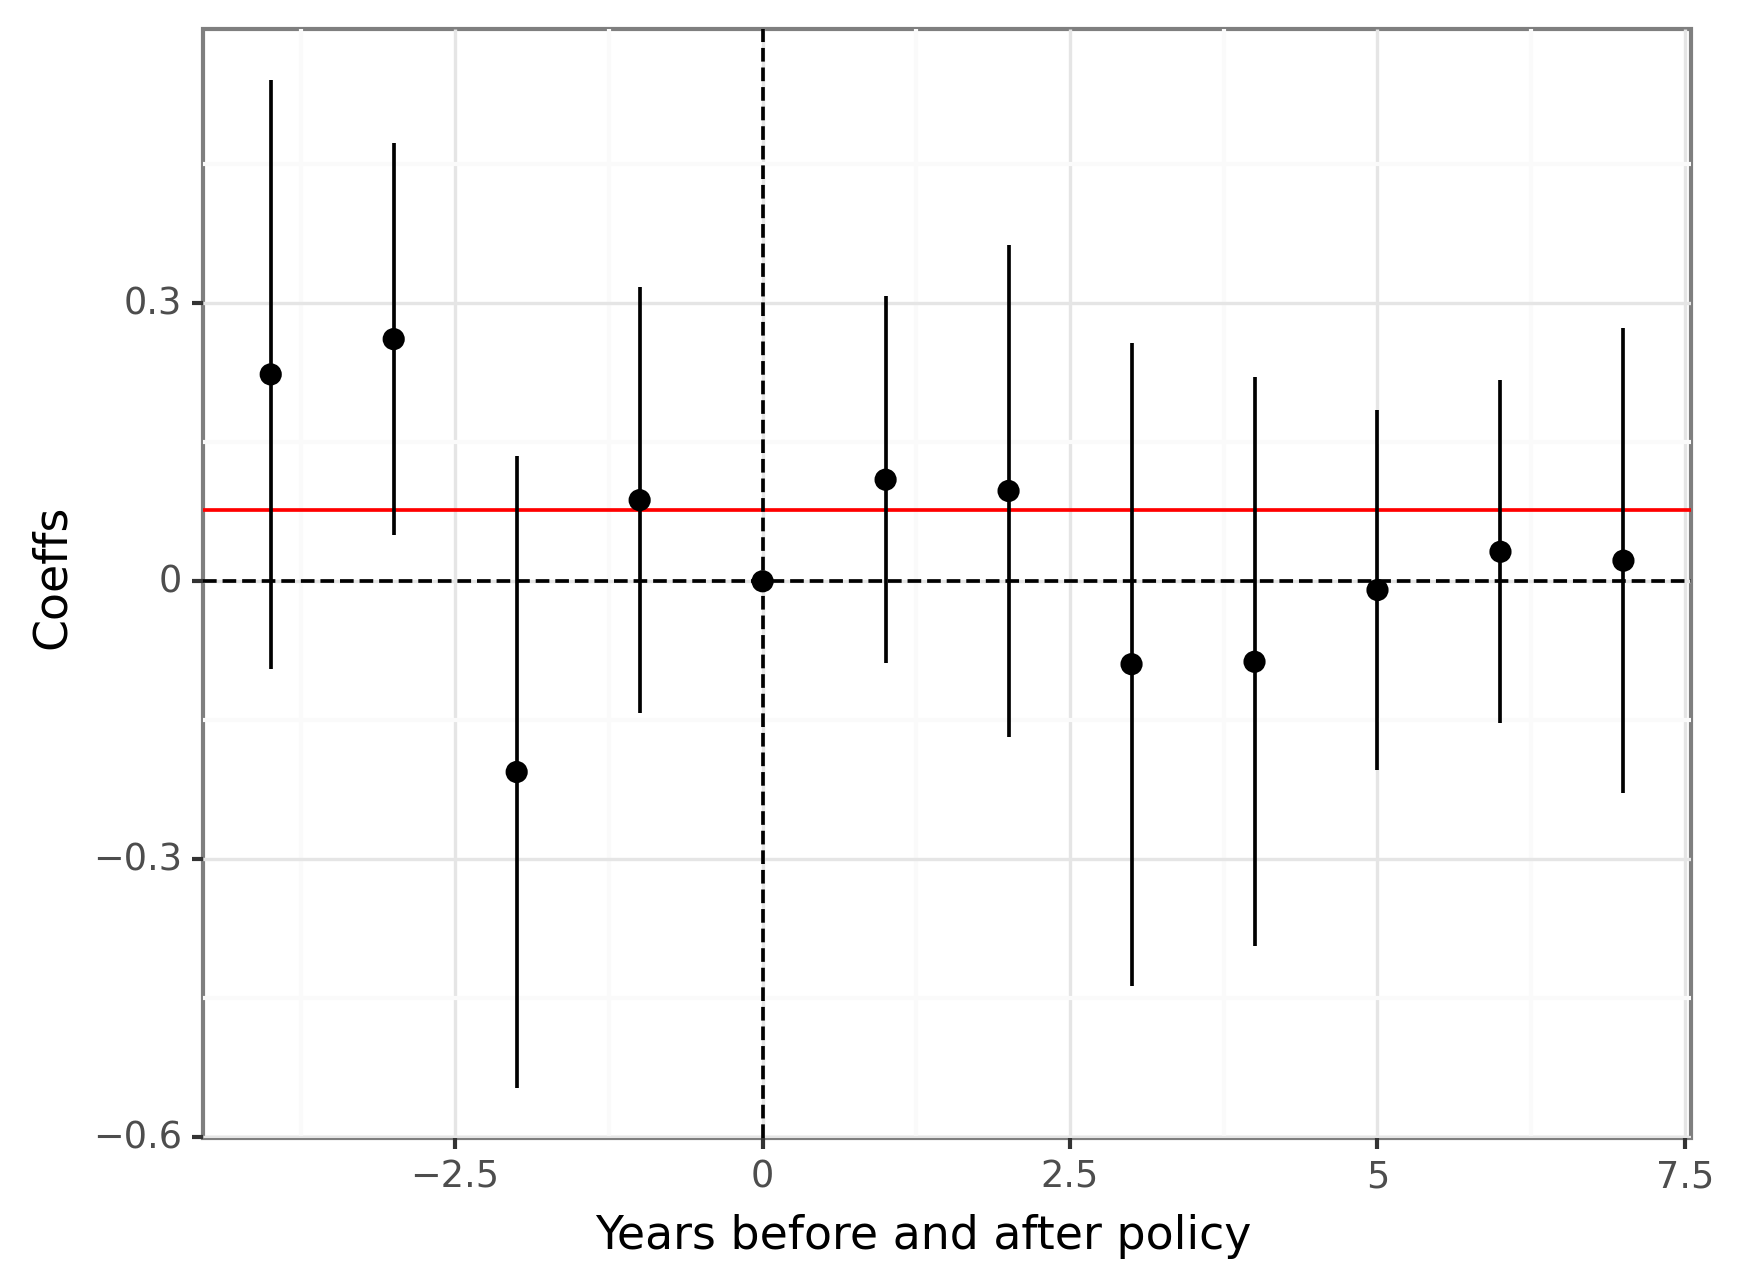
\includegraphics[width=0.85\textwidth]{../bld/python/figures/event_study_gym}
     \caption{Event Study plot with leads and lags}\label{fig:event_study}
\end{figure}

\subsection{Main results}
Table\ref{tab:main_reg} presents the estimates of equation (\ref{eqn:main_eqn}). Using the controls as shown in the table I get highly significant result. The controls is 
similar to the paper by \citep{dohmen2008representative}. Although the study was not related to G8 reform Yet it showed women have more trust as contrary to the result present
here. The negative effect for females on the other side could be because of the differential impact the reform had for boys and girls, with the latter often experiencing a 
decline in school performance \citep{dahmann2017does}. Significant effects for students with higher educated parents and those with a working-class father. While the former 
in general exhibit a substantially higher degree of trust, the latter trust less what could be related to less support these children receive at home to cope with the increased 
pressure at school as proposed by \citet{dahmann2014impact}. Overall, it can be seen that the reform had an important and significantly sizeable effect on student's self rated trust. 

\subsection{Mechanisms}
In this project I tries to look into the mechanisms which might cause the increse in trust.Tables\ref{tab:mech_sport_active},\ref{tab:mech_vw} shows the results. Although no significant 
results were found may be beacuse of the lower sample size. Althogh postive it shows low impact for treated. There are researches which have shown low impact of the leisure time activites 
of children due incresed pressure. There are many other mechanisms which can be explored like the "Bive-five" as a mechanism design which I am yet to explore. Or any other in-school programes
but the data set used does not contain such information. 

\subsection{Robust Check}
Since trust was measured in the likert scale, here I used the ordered logit model to check the robustness of the main regression model, it can be expected to receive better or similar result.
Table\ref{tab:robustness} shows the trust is still significant which hints to the fact the main regression is robust to model slection. There is possibility to also check the palcebo by 
looking at the trust attitude of the non-gymnasium students which is yet to be explored.  

\section{Conclusion\label{sec:conclusion}}
Drawing on data from the SOEP and using a difference-in-differences design,it is hown that the reform led to a
significant increase in self rated trust of almost 0.15 of a standard deviation with significant differential
effects emerging for students with less educated parents or those being considered as low-performing.
Investigate some potential mechanisms, including changes in time allocation and school-related
changes and it appears to be the case that our result was driven by school-related characteristics which
could not be entirely captured with our data. In addtition extending gratitude to\citep{GaudeckerEconProjectTemplates}
for the project template making the work easier. 









\setstretch{1}
%\nocite{*}
\printbibliography
\setstretch{1.5}



\section{Appendix\label{sec:appendix}}

\begin{figure}[H]
    \centering
    \includegraphics[width=0.85\textwidth]{../bld/python/figures/descriptive_stats.png}
     \caption{Descriptive statistics by treatment status}\label{fig:descriptive_stats}
\end{figure}

%\begin{table}[!h]
\begin{table}[H]
    \input{../bld/python/tables/main_regression.tex}
    \caption{\label{tab:main_reg}\emph{Python:} Estimation results of the
        main two way fixed effect regression.}
\end{table}

\begin{table}[H]
    \begin{center}
\begin{tabular}{lclc}
\toprule
\textbf{Dep. Variable:}                  & volunteer\_work  & \textbf{  R-squared:         } &     0.656   \\
\textbf{Model:}                          &       OLS        & \textbf{  Adj. R-squared:    } &     0.190   \\
\textbf{Method:}                         &  Least Squares   & \textbf{  F-statistic:       } & -2.029e+13  \\
\textbf{Date:}                           & Wed, 22 Mar 2023 & \textbf{  Prob (F-statistic):} &     1.00    \\
\textbf{Time:}                           &     18:59:01     & \textbf{  Log-Likelihood:    } &   -6.2893   \\
\textbf{No. Observations:}               &          34      & \textbf{  AIC:               } &     52.58   \\
\textbf{Df Residuals:}                   &          14      & \textbf{  BIC:               } &     83.11   \\
\textbf{Df Model:}                       &          19      & \textbf{                     } &             \\
\textbf{Covariance Type:}                &     cluster      & \textbf{                     } &             \\
\bottomrule
\end{tabular}
\begin{tabular}{lcccccc}
                                         & \textbf{coef} & \textbf{std err} & \textbf{z} & \textbf{P$> |$z$|$} & \textbf{[0.025} & \textbf{0.975]}  \\
\midrule
\textbf{Intercept}                       &       0.0004  &        0.004     &     0.080  &         0.936        &       -0.008    &        0.009     \\
\textbf{C(year\_hgsch\_entry)[T.2001.0]} &      -0.9434  &        0.595     &    -1.586  &         0.113        &       -2.109    &        0.222     \\
\textbf{C(year\_hgsch\_entry)[T.2003.0]} &      -2.4198  &        0.273     &    -8.865  &         0.000        &       -2.955    &       -1.885     \\
\textbf{C(year\_hgsch\_entry)[T.2004.0]} &      -1.0000  &     1.94e-08     & -5.15e+07  &         0.000        &       -1.000    &       -1.000     \\
\textbf{C(year\_hgsch\_entry)[T.2005.0]} &      -1.5696  &        0.136     &   -11.563  &         0.000        &       -1.836    &       -1.304     \\
\textbf{C(year\_hgsch\_entry)[T.2006.0]} &      -1.3779  &        0.091     &   -15.105  &         0.000        &       -1.557    &       -1.199     \\
\textbf{C(year\_hgsch\_entry)[T.2007.0]} &      -1.2965  &        0.177     &    -7.321  &         0.000        &       -1.644    &       -0.949     \\
\textbf{C(year\_hgsch\_entry)[T.2008.0]} &      -1.4802  &        0.272     &    -5.438  &         0.000        &       -2.014    &       -0.947     \\
\textbf{C(year\_hgsch\_entry)[T.2009.0]} &      -0.9583  &        0.587     &    -1.634  &         0.102        &       -2.108    &        0.191     \\
\textbf{C(year\_hgsch\_entry)[T.2010.0]} &      -0.4473  &        0.556     &    -0.804  &         0.421        &       -1.537    &        0.642     \\
\textbf{C(year\_hgsch\_entry)[T.2011.0]} &      -1.2217  &        0.472     &    -2.586  &         0.010        &       -2.148    &       -0.296     \\
\textbf{C(year\_hgsch\_entry)[T.2012.0]} &      -0.9062  &        0.599     &    -1.513  &         0.130        &       -2.080    &        0.268     \\
\textbf{Treat}                           &       1.0000  &          nan     &       nan  &           nan        &          nan    &          nan     \\
\textbf{Age}                             &       0.0061  &        0.076     &     0.080  &         0.936        &       -0.144    &        0.156     \\
\textbf{female}                          &       0.4070  &        0.354     &     1.149  &         0.251        &       -0.287    &        1.101     \\
\textbf{rural}                           &   -9.459e-16  &      2.2e-16     &    -4.290  &         0.000        &    -1.38e-15    &    -5.14e-16     \\
\textbf{East}                            &       0.4198  &        0.273     &     1.538  &         0.124        &       -0.115    &        0.955     \\
\textbf{low\_performing}                 &      -0.1237  &        0.199     &    -0.622  &         0.534        &       -0.514    &        0.266     \\
\textbf{highest\_educ\_hh}               &       0.2510  &        0.235     &     1.069  &         0.285        &       -0.209    &        0.711     \\
\textbf{migration\_backgrnd}             &       0.0004  &        0.004     &     0.080  &         0.936        &       -0.008    &        0.009     \\
\textbf{work\_father}                    &       0.1233  &        0.336     &     0.367  &         0.714        &       -0.536    &        0.783     \\
\textbf{work\_mother}                    &      -0.0863  &        0.321     &    -0.269  &         0.788        &       -0.716    &        0.543     \\
\textbf{reli\_hh}                        &       0.3237  &        0.572     &     0.566  &         0.572        &       -0.798    &        1.445     \\
\bottomrule
\end{tabular}
\begin{tabular}{lclc}
\textbf{Omnibus:}       &  3.020 & \textbf{  Durbin-Watson:     } &    1.480  \\
\textbf{Prob(Omnibus):} &  0.221 & \textbf{  Jarque-Bera (JB):  } &    2.100  \\
\textbf{Skew:}          &  0.603 & \textbf{  Prob(JB):          } &    0.350  \\
\textbf{Kurtosis:}      &  3.170 & \textbf{  Cond. No.          } & 5.28e+18  \\
\bottomrule
\end{tabular}
%\caption{OLS Regression Results}
\end{center}

Notes: \newline
 [1] Standard Errors are robust to cluster correlation (cluster) \newline
 [2] The smallest eigenvalue is 3.58e-34. This might indicate that there are \newline
 strong multicollinearity problems or that the design matrix is singular.

    \caption{\label{tab:mech_vw}\emph{Python:} Mechanism- Volunteer work (outside school)}
\end{table}

\begin{table}[H]
    \begin{center}
\begin{tabular}{lclc}
\toprule
\textbf{Dep. Variable:}       &  sport\_active   & \textbf{  R-squared:         } &     0.027   \\
\textbf{Model:}               &       OLS        & \textbf{  Adj. R-squared:    } &     0.018   \\
\textbf{Method:}              &  Least Squares   & \textbf{  F-statistic:       } &     34.46   \\
\textbf{Date:}                & Mon, 27 Mar 2023 & \textbf{  Prob (F-statistic):} &  3.97e-08   \\
\textbf{Time:}                &     17:05:16     & \textbf{  Log-Likelihood:    } &   -441.99   \\
\textbf{No. Observations:}    &        1089      & \textbf{  AIC:               } &     906.0   \\
\textbf{Df Residuals:}        &        1078      & \textbf{  BIC:               } &     960.9   \\
\textbf{Df Model:}            &          10      & \textbf{                     } &             \\
\textbf{Covariance Type:}     &     cluster      & \textbf{                     } &             \\
\bottomrule
\end{tabular}
\begin{tabular}{lcccccc}
                              & \textbf{coef} & \textbf{std err} & \textbf{z} & \textbf{P$> |$z$|$} & \textbf{[0.025} & \textbf{0.975]}  \\
\midrule
\textbf{Intercept}            &       0.8846  &        0.049     &    17.937  &         0.000        &        0.788    &        0.981     \\
\textbf{Treat}                &       0.0123  &        0.019     &     0.649  &         0.516        &       -0.025    &        0.049     \\
\textbf{female}               &      -0.0532  &        0.017     &    -3.091  &         0.002        &       -0.087    &       -0.019     \\
\textbf{East}                 &      -0.0942  &        0.038     &    -2.446  &         0.014        &       -0.170    &       -0.019     \\
\textbf{low\_performing}      &      -0.0596  &        0.024     &    -2.447  &         0.014        &       -0.107    &       -0.012     \\
\textbf{highest\_educ\_hh}    &       0.0540  &        0.021     &     2.510  &         0.012        &        0.012    &        0.096     \\
\textbf{work\_father}         &      -0.0243  &        0.035     &    -0.693  &         0.488        &       -0.093    &        0.044     \\
\textbf{work\_mother}         &       0.0103  &        0.024     &     0.429  &         0.668        &       -0.037    &        0.057     \\
\textbf{reli\_hh}             &      -0.0324  &        0.021     &    -1.564  &         0.118        &       -0.073    &        0.008     \\
\textbf{single\_parent}       &      -0.0002  &        0.027     &    -0.009  &         0.993        &       -0.053    &        0.053     \\
\textbf{migration\_classmate} &      -0.0176  &        0.022     &    -0.796  &         0.426        &       -0.061    &        0.026     \\
\bottomrule
\end{tabular}
\begin{tabular}{lclc}
\textbf{Omnibus:}       & 317.763 & \textbf{  Durbin-Watson:     } &     1.974  \\
\textbf{Prob(Omnibus):} &   0.000 & \textbf{  Jarque-Bera (JB):  } &   650.155  \\
\textbf{Skew:}          &  -1.771 & \textbf{  Prob(JB):          } & 6.62e-142  \\
\textbf{Kurtosis:}      &   4.337 & \textbf{  Cond. No.          } &      11.5  \\
\bottomrule
\end{tabular}
%\caption{OLS Regression Results}
\end{center}

Notes: \newline
 [1] Standard Errors are robust to cluster correlation (cluster)
    \caption{\label{tab:mech_sport_active}\emph{Python:} Mechanism- School sport(inside school)}
\end{table}

\begin{table}[H]
    \input{../bld/python/tables/placebo_regression.tex}
    \caption{\label{tab:robustness}\emph{Python:} Robustcheck}
\end{table}

% \setstretch{1}
% %\nocite{*}
% \printbibliography
% \setstretch{1.5}

\end{document}


% section introduction (end)

% \clearpage
% \begin{singlespace}
% %\bibliographystyle{plainnat}
% %\bibliographystyle{chicago}
% \bibliographystyle{aer}
% \bibliography{../../paper/refs.bib}
% \end{singlespace}

% \setstretch{1}
% \printbibliography{}
% \setstretch{1.5}



% \appendix

% The chngctr package is needed for the following lines.
% \counterwithin{table}{section}
% \counterwithin{figure}{section}


